% !TeX root = ICCPS18.tex
\section{Experimental Evaluation and Discussions}
\label{sec:results}

We consider a collection of load traces recorded by Siemens from a microgrid in Germany, containing $102$ homes across $11$ feeders ($5$ producers and $97$ consumers). %Table \ref{tab:prosumers}
Figure~\ref{fig:feeder} describes the feeder structure, the number of participants per feeder, and  the feeder safety limits. We use $\Delta =15$ minute intervals, resulting in a total of $96$ intervals across the whole day.   Figure~\ref{fig:profile} shows the total production and consumption across this microgrid. The horizontal axis shows the starting time for each of the $96$ intervals. 
\AronC{I added this to address the lack of prices in our }
Since the dataset does not include prices, we assume reservation prices to be uniform in our experiments, and focus on studying the amount of energy traded and the performance of the system.

As one of our primary contributions in this work is the ability to specify multiple time intervals for  selling offers, we extended the trace that was collected by Siemens to allow each producer to have a battery with a total capacity of $90$ kWh. With a battery, a producer can take the energy produced in  a time interval and decide to make it available in future time intervals.
Note that the resulting offers always span a contiguous set of time intervals, so they can be specified by their starting time and length. 
Figure \ref{fig:batteryEffect} shows these intervals for one particular producer. The producers charge their batteries only when the total consumption is less than the total production, which happens just after 12:00 PM, see Figure~\ref{fig:profile}.


% !TeX root = ICCPS18.tex
   
     \begin{figure}[t]
 \centering
\resizebox{0.45\textwidth}{!}{%
 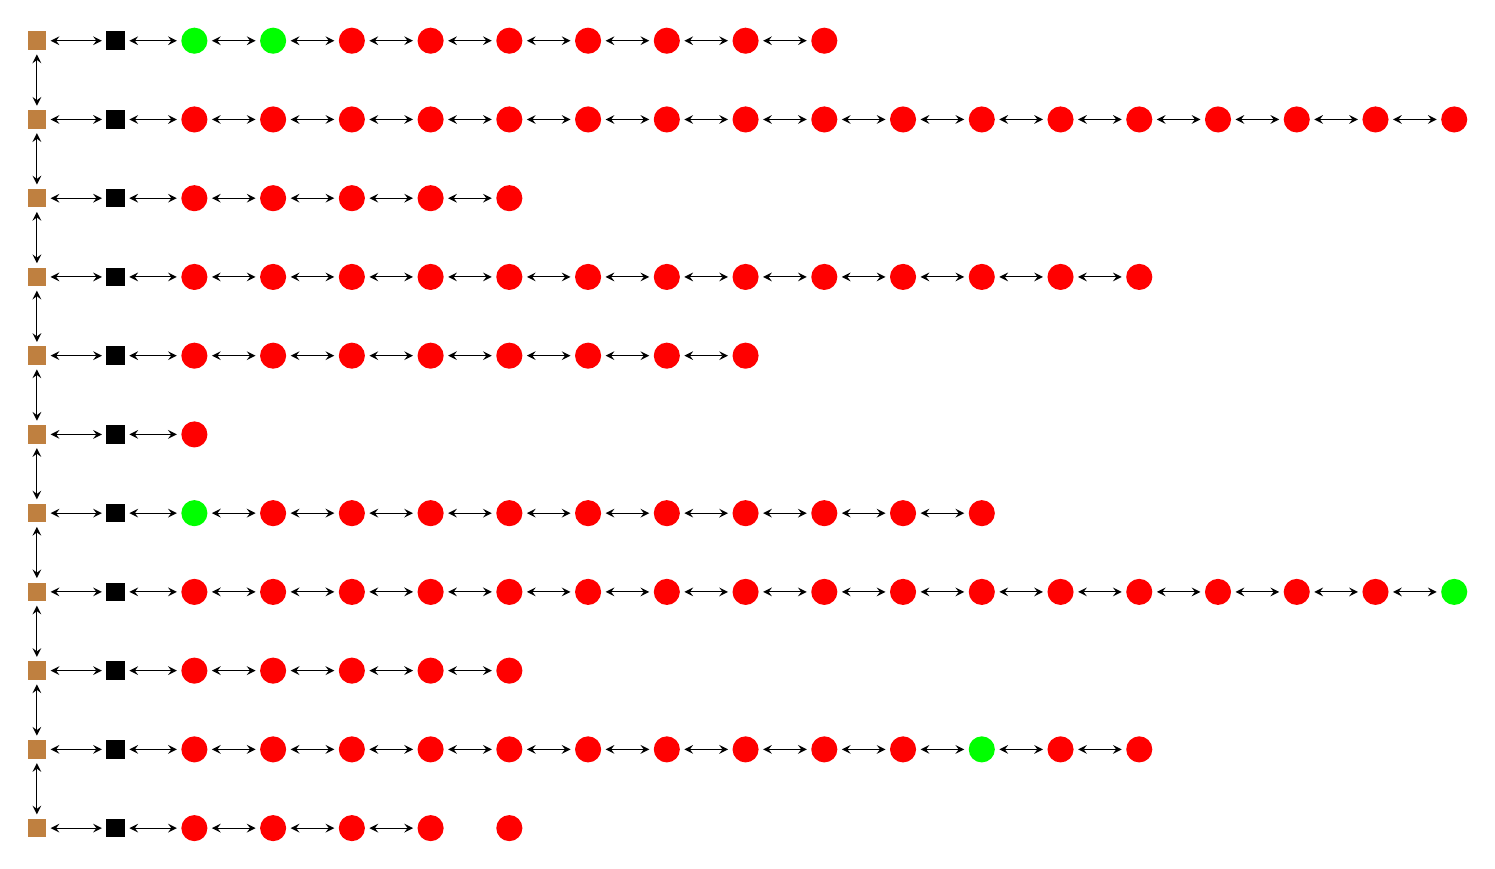
\begin{tikzpicture}[rotate=270,font=\tiny,
   oc/.style={fill=black,rectangle,minimum size=0.01cm,font=\tiny},
     feeder/.style={fill=brown,rectangle,minimum size=0.005cm,font=\tiny},
   Producer/.style={fill=green,circle,minimum size=0.01cm},
     Consumer/.style={fill=red,circle,minimum size=0.01cm},
   Connection/.style={<->, >=stealth, shorten <=0.05cm, shorten >=0.05cm}]
 \draw node[oc] (oc1) at (-5,0){};
 \draw node[oc] (oc2) at (-4,0){};
 \draw node[oc] (oc3) at (-3,0){};
 \draw node[oc] (oc4)  at (-2,0){};
 \draw node[oc](oc5)  at (-1,0){};
 \draw node[oc] (oc6)  at (0,0){};
 \draw node[oc] (oc7) at (1,0){};
 \draw node[oc] (oc8)  at (2,0){};
 \draw node[oc] (oc9) at (3,0){};
 \draw node[oc] (oc10) at (4,0){};
 \draw node[oc] (oc11) at (5,0){};

 \draw node[feeder] (feeder1) at (-5,-1){};
 \draw node[feeder] (feeder2) at (-4,-1){};
 \draw node[feeder] (feeder3) at (-3,-1){};
 \draw node[feeder] (feeder4)  at (-2,-1){};
 \draw node[feeder](feeder5)  at (-1,-1){};
 \draw node[feeder] (feeder6)  at (0,-1){};
 \draw node[feeder] (feeder7) at (1,-1){};
 \draw node[feeder] (feeder8)  at (2,-1){};
 \draw node[feeder] (feeder9) at (3,-1){};
 \draw node[feeder] (feeder10) at (4,-1){};
 \draw node[feeder] (feeder11) at (5,-1){};

 \draw [Connection] (feeder1) to (feeder2);
 \draw [Connection] (feeder2) to (feeder3);
 \draw [Connection] (feeder3) to (feeder4);
 \draw [Connection] (feeder4) to (feeder5);
 \draw [Connection] (feeder5) to (feeder6);
 \draw [Connection] (feeder6) to (feeder7);
 \draw [Connection] (feeder7) to (feeder8);
 \draw [Connection] (feeder8) to (feeder9);
 \draw [Connection] (feeder9) to (feeder10);
 \draw [Connection] (feeder10) to (feeder11);

\draw [Connection] (feeder1) to (oc1);
\draw [Connection] (feeder2) to (oc2);
\draw [Connection] (feeder3) to (oc3);
\draw [Connection] (feeder4) to (oc4);
\draw [Connection] (feeder5) to (oc5);
\draw [Connection] (feeder6) to (oc6);
\draw [Connection] (feeder7) to (oc7);
\draw [Connection] (feeder8) to (oc8);
\draw [Connection] (feeder9) to (oc9);
\draw [Connection] (feeder10) to (oc10);
\draw [Connection] (feeder11) to (oc11);


 \foreach \pos in {1,2} {
   \node [Producer] (p10\pos)at (-5,\pos) {};
 }

 \foreach \pos in {3,4,5,6,7,8,9} {
   \node [Consumer] (c10\pos)at (-5,\pos) {};
 }

 \foreach \pos in {1,2,3,4,5,6,7,8,9,10,11,12,13,14,15,16,17} {
   \node [Consumer] (c20\pos)at (-4,\pos) {};
 }

 \foreach \pos in {1,2,3,4,5} {
   \node [Consumer] (c30\pos)at (-3,\pos) {};
 }


 \foreach \pos in {1,2,3,4,5,6,7,8,9,10,11,12,13} {
   \node [Consumer] (c40\pos)at (-2,\pos) {};
 }


 \foreach \pos in {1,2,3,4,5,6,7,8} {
   \node [Consumer] (c50\pos)at (-1,\pos) {};
 }


 \foreach \pos in {1} {
   \node [Consumer] (c60\pos)at (0,\pos) {};
 }


 \foreach \pos in {1} {
   \node [Producer] (p70\pos)at (1,\pos) {};
 }


 \foreach \pos in {2,3,4,5,6,7,8,9,10,11} {
   \node [Consumer] (c70\pos)at (1,\pos) {};
 }


 \foreach \pos in {17} {
   \node [Producer] (p80\pos)at (2,\pos) {};
 }

 \foreach \pos in {1,2,3,4,5,6,7,8,9,10,11,12,13,14,15,16} {
   \node [Consumer] (c80\pos)at (2,\pos) {};
 }

 \foreach \pos in {1,2,3,4,5} {
   \node [Consumer] (c90\pos)at (3,\pos) {};
 }

 \foreach \pos in {11} {
   \node [Producer] (p100\pos)at (4,\pos) {};
 }

 \foreach \pos in {1,2,3,4,5,6,7,8,9,10,12,13} {
   \node [Consumer] (c100\pos)at (4,\pos) {};
 }

 \foreach \pos in {1,2,3,4,5} {
   \node [Consumer] (c110\pos)at (5,\pos) {};
 }


 \draw [Connection] (oc1) to (p101);
 \draw [Connection] (p101) to (p102);
 \draw [Connection] (p102) to (c103);
 \draw [Connection] (c103) to (c104);
 \draw [Connection] (c104) to (c105);
 \draw [Connection] (c105) to (c106);
 \draw [Connection] (c106) to (c107);
 \draw [Connection] (c107) to (c108);
 \draw [Connection] (c108) to (c109);
 
\draw [Connection] (oc2) to (c201);
\draw [Connection] (c201) to (c202);
\draw [Connection] (c202) to (c203);
\draw [Connection] (c203) to (c204);
\draw [Connection] (c204) to (c205);
\draw [Connection] (c205) to (c206);
\draw [Connection] (c206) to (c207);
\draw [Connection] (c207) to (c208);
\draw [Connection] (c208) to (c209);
\draw [Connection] (c209) to (c2010);
\draw [Connection] (c2010) to (c2011);
\draw [Connection] (c2011) to (c2012);
\draw [Connection] (c2012) to (c2013);
\draw [Connection] (c2013) to (c2014);
\draw [Connection] (c2014) to (c2015);
\draw [Connection] (c2015) to (c2016);
\draw [Connection] (c2016) to (c2017);

\draw [Connection] (oc3) to (c301);
\draw [Connection] (c301) to (c302);
\draw [Connection] (c302) to (c303);
\draw [Connection] (c303) to (c304);
\draw [Connection] (c304) to (c305);

\draw [Connection] (oc4) to (c401);
\draw [Connection] (c401) to (c402);
\draw [Connection] (c402) to (c403);
\draw [Connection] (c403) to (c404);
\draw [Connection] (c404) to (c405);
\draw [Connection] (c405) to (c406);
\draw [Connection] (c406) to (c407);
\draw [Connection] (c407) to (c408);
\draw [Connection] (c408) to (c409);
\draw [Connection] (c409) to (c4010);
\draw [Connection] (c4010) to (c4011);
\draw [Connection] (c4011) to (c4012);
\draw [Connection] (c4012) to (c4013);

\draw [Connection] (oc5) to (c501);
\draw [Connection] (c501) to (c502);
\draw [Connection] (c502) to (c503);
\draw [Connection] (c503) to (c504);
\draw [Connection] (c504) to (c505);
\draw [Connection] (c505) to (c506);
\draw [Connection] (c506) to (c507);
\draw [Connection] (c507) to (c508);

\draw [Connection] (oc6) to (c601);

\draw [Connection] (oc7) to (p701);
\draw [Connection] (p701) to (c702);
\draw [Connection] (c702) to (c703);
\draw [Connection] (c703) to (c704);
\draw [Connection] (c704) to (c705);
\draw [Connection] (c705) to (c706);
\draw [Connection] (c706) to (c707);
\draw [Connection] (c707) to (c708);
\draw [Connection] (c708) to (c709);
\draw [Connection] (c709) to (c7010);
\draw [Connection] (c7010) to (c7011);

\draw [Connection] (oc8) to (c801);
\draw [Connection] (c801) to (c802);
\draw [Connection] (c802) to (c803);
\draw [Connection] (c803) to (c804);
\draw [Connection] (c804) to (c805);
\draw [Connection] (c805) to (c806);
\draw [Connection] (c806) to (c807);
\draw [Connection] (c807) to (c808);
\draw [Connection] (c808) to (c809);
\draw [Connection] (c809) to (c8010);
\draw [Connection] (c8010) to (c8011);
\draw [Connection] (c8011) to (c8012);
\draw [Connection] (c8012) to (c8013);
\draw [Connection] (c8013) to (c8014);
\draw [Connection] (c8014) to (c8015);
\draw [Connection] (c8015) to (c8016);
\draw [Connection] (c8016) to (p8017);

\draw [Connection] (oc9) to (c901);
\draw [Connection] (c901) to (c902);
\draw [Connection] (c902) to (c903);
\draw [Connection] (c903) to (c904);
\draw [Connection] (c904) to (c905);

\draw [Connection] (oc10) to (c1001);
\draw [Connection] (c1001) to (c1002);
\draw [Connection] (c1002) to (c1003);
\draw [Connection] (c1003) to (c1004);
\draw [Connection] (c1004) to (c1005);
\draw [Connection] (c1005) to (c1006);
\draw [Connection] (c1006) to (c1007);
\draw [Connection] (c1007) to (c1008);
\draw [Connection] (c1008) to (c1009);
\draw [Connection] (c1009) to (c10010);
\draw [Connection] (c10010) to (p10011);
\draw [Connection] (p10011) to (c10012);
\draw [Connection] (c10012) to (c10013);


\draw [Connection] (oc11) to (c1101);
\draw [Connection] (c1101) to (c1102);
\draw [Connection] (c1102) to (c1103);
\draw [Connection] (c1103) to (c1104);

 \end{tikzpicture}
 }
 \caption{Feeder diagram. Brown nodes are feeder junctions, numbered 1 to 11 from top to bottom.  Black nodes are the overcurrent relays, which ensure that the total power flowing in and out of the feeder is below 20 kW. The green nodes are the junction points for the producers ($5$), and the red nodes are junction points for the consumers ($97$). There are $102$ prosumers in total.}
 \label{fig:feeder}
 \end{figure}


\begin{figure}[t]
\centering
\begin{tikzpicture}
\begin{axis}[
  font=\footnotesize,
  width=\columnwidth,
  height=0.61\columnwidth,
  ymin=-1,
 legend columns=3, 
  legend style={font=\fontsize{5}{6}\selectfont,cells={align=left},text width=4.3em,text height=1.5ex,text depth=.5ex,row sep=0.1em},
  ymax=220,
grid=both,
    grid style={line width=.1pt, draw=gray!10},
    major grid style={line width=.2pt,draw=gray!50},
  xmin=-1,
  xmax=97,
  legend pos=north west,
  xlabel=Time,
  ylabel={[kWh]},
  ytick={0, 50, 100, 150, 200},
  xtick={0, 16, 32, 48, 64, 80, 95},
  xticklabels={0:00, 4:00, 8:00, 12:00, 16:00,  20:00, 23:45},
]
\addplot[no markers, solid, greenline, semithick] table[x expr=\coordindex, y=WithoutBattery,  comment chars={\%}, col sep=comma] {diagrams/interval-energy-traded.csv};
\addlegendentry{Total energy traded (Test A)};
\addplot[no markers, solid, blackLine, semithick] table[x expr=\coordindex, y=WithBattery5,  comment chars={\%}, col sep=comma] {diagrams/interval-energy-traded.csv};
\addlegendentry{Total energy traded (Test C)};
\addplot[no markers, solid, goldLine, semithick] table[x expr=\coordindex, y=WithBattery12,  comment chars={\%}, col sep=comma] {diagrams/interval-energy-traded.csv};
\addlegendentry{Total energy traded (Test D)};
\addplot[no markers, solid, blueLine, semithick] table[x expr=\coordindex, y=TotalProduction, comment chars={\%}] {diagrams/TotalProductionConsumption.csv};
\addlegendentry{Total production};
\addplot[no markers, solid, redLine, semithick] table[x expr=\coordindex, y=TotalConsumption, comment chars={\%}] {diagrams/TotalProductionConsumption.csv};
\addlegendentry{Total consumption};
\end{axis}
\end{tikzpicture}
\caption{Load profile (i.e., total consumption) and generation profile (i.e., total production) in kWh per 15 minute interval aggregated across the microgrid.  The graph also shows the energy traded per interval without battery, with battery and prediction window of 5 intervals, and with battery and prediction window of 12 intervals. Note that the amount of energy traded can be lower than both demand and supply at the same time because of safety constraints, which limit the amount of energy that can flow out of the producers' feeders.}
\label{fig:profile}
% \vspace{-0.2in}
\end{figure}



\begin{figure}[ht]
\begin{tikzpicture}
\begin{axis}[
  font=\footnotesize,
  width=0.94\columnwidth,
  height=0.65\columnwidth,
  ymin=-0.2,
  ymax=10,
  xmin=28,
  xmax=95,
  ylabel={Energy [kWh]},
  xtick={0, 16, 32, 48, 64, 80, 95},
  xticklabels={0:00, 4:00, 8:00, 12:00, 16:00,  20:00, 23:45},
grid=both,
    grid style={line width=.1pt, draw=gray!10},
    major grid style={line width=.2pt,draw=gray!50},
]
\addplot[mark=*, mark size=0.5, solid, blueLine, semithick] table[x= startTime, y=Energy, comment chars={\%}] {diagrams/outputTestA.csv};
\end{axis}
\begin{axis}[
  font=\footnotesize,
  width=0.94\columnwidth,
  height=0.65\columnwidth,
  ymin=-1,
  ymax=50,
  xmin=28,
  xmax=95,
  xtick={},
  xticklabels={},
  ylabel={Offer length [intervals]},
  ytick={0, 10, 20, 30, 40, 50},
  axis y line*=right,
  legend pos=north east,
]
\addlegendimage{blueLine, semithick}
\addlegendentry{Energy}
\addplot[ybar interval,redLine] table[ x=startTime,y=Availability, comment chars={\%}] {diagrams/outputTestA.csv};
\addlegendentry{Offer length}
\end{axis}
\end{tikzpicture}
\caption{Energy offered in each time interval by the first prosumer of the first feeder when using a battery (blue line). The red bars indicate the number of contiguous intervals for which the offer is valid. The total battery capacity is 90 kWh. It is assumed that the battery charges at a rate of 10 kWh per interval. Producers are assumed to keep the battery available till the end of the test, which is the 95th interval. Consequently, the red bars taper off in consecutive intervals.}
\label{fig:batteryEffect}
\end{figure}

 
 \begin{figure}[ht]
	\centering		\includegraphics[width=1\columnwidth]{diagrams/testbed.jpg}
	\caption{Hardware test bed.}
   \label{fig:testbed_architecture}
\end{figure}


\begin{table}[ht]    
%\setlength{\tabcolsep}{4pt}
\caption{Parameter Values for Experiments (See Table \ref{tab:symbols})}
\label{table:test-parameters}  
\centering
\begin{tabular}{lllll}
& A  & B  & C  & D     \\ \cline{2-5} 
\multicolumn{1}{l|}{$\Delta$[m]}   & 15 & 15 & 15 & 15   \\
\multicolumn{1}{l|}{$\Delta_s$ [s]}   & 5 & 5 & 5 & 5   \\
\multicolumn{1}{l|}{$\hat{\Delta}$ [s]} & 120 & 120 & 120 & 120   \\
\multicolumn{1}{l|}{$L$}          & 2,3,5,7,10,13  & 2,3,7,10  & 5  & 13    \\
\multicolumn{1}{l|}{Battery}     & no & yes & yes & yes \\
\hline
\multicolumn{1}{l|}{Figure}     & \ref{fig:multihorizon} &\ref{fig:multihorizon} & \ref{fig:allocate1NRG},\ref{fig:time},\ref{fig:profile},\ref{fig:multihorizon} &  \ref{fig:profile},\ref{fig:multihorizon} 
\end{tabular}
\end{table}






\begin{figure}[ht]
\begin{tikzpicture}
\begin{axis}[
  font=\footnotesize,
  width=\columnwidth,
  height=0.61\columnwidth,
  ymin=2865,
  ymax=2975,
  ytick={2875,2900,2925,2950},
  xtick={2,3,5,7,10,13},
  legend pos=north west,
  xlabel={Prosumer prediction window [time intervals]},
  ylabel={Total energy traded [kWh]},
grid=both,
    grid style={line width=.1pt, draw=gray!10},
    major grid style={line width=.2pt,draw=gray!50},
]
\addplot[mark=o, color=blueLine, only marks, thick] table[x=predictionWindow, y=withoutBattery, comment chars={\%}, col sep=comma] {diagrams/total-energy-traded.csv};
\addlegendentry{without battery};
\addplot[mark=+, color=redLine, only marks, thick] table[x=predictionWindow, y=withBattery, comment chars={\%}, col sep=comma] {diagrams/total-energy-traded.csv};
\addlegendentry{with battery};
\end{axis}
\end{tikzpicture}
\caption{Total amount of energy traded in the entire microgrid with and without batteries, for various prediction window lengths.}
\label{fig:multihorizon}
\end{figure}


\begin{figure}[t]
	\centering
\includegraphics[width=1\columnwidth]{diagrams/prosumer101.pdf}
	\caption{Energy generated in each interval (blue line) and energy traded to a set of consumers in each interval (vertical bars) for the first prosumer of the first feeder (Test case C). The stacked colors show the different consumers that were matched with the prosumer in each interval (note that the same color across multiple intervals does not necessarily mean the same consumer). When the energy traded exceeds the generation, the excess is drawn from the battery.}
	\label{fig:allocate1NRG}
\end{figure}

\begin{figure}[htb]
	\centering
    \begin{tikzpicture}
    	\begin{axis}[
	width=\columnwidth,
	height=0.5\columnwidth,
	bar width=0.04\textwidth,
    font=\footnotesize,
    grid=both,
    grid style={line width=.1pt, draw=gray!10},
    major grid style={line width=.2pt,draw=gray!50},
	ybar,
	ytick={0, 5, 10, 15, 20},
	%yticklabels={40, 60, 90, 135},
	xlabel style={align=center},
	xlabel={Real time [seconds]},
	ylabel={Number of Offers},
	symbolic x coords={0,1,2,3,4,5},
	xticklabels={{[11, 23]}, {(23, 35]}, {(35, 47]}, {(47, 59]}, {(59, 71]}, {(71, 84]}},
	xtick=data,
	ylabel style={align=center},
	]
\addplot[fill=blueFill] coordinates { 
		(0, 20)
		(1, 20)
		(2, 12)
		(3, 5)
		(4, 1)
		(5, 1)
	};
	\end{axis}
\end{tikzpicture}
%\includegraphics[width=1\columnwidth]{diagrams/timechart.pdf}
	\caption{Real time in seconds between posting an offer and recording a trade that includes the offer (Test case C). This time includes the communication delay, the time to mine the blockchain, and the running time required to find a solution. Since the solver runs periodically and receives offers asynchronously, there might be a few runs before a suitable match is found.}
	\label{fig:time}
\end{figure}


%\textcolor{red}{Table ... describes our data conversion rules.}







\subsection{Test Bed}
The hardware test bed is a cluster of 31 BeagleBone Black~\footnote{https://beagleboard.org/black} (BBB)  single-board computers (see Figure~\ref{fig:testbed_architecture}) acting as participants in the energy trading system. The BBBs are set up as light clients because they are resource constrained and therefore are not suitable for mining or acting as solvers. This means that they can safely access the blockchain but do not participate in the consensus process.  In the dataset provided by Siemens, there are 95 consumers and 7 producers of power,  see Figure \ref{fig:components}. These participants are divided between the BBBs in the cluster. The  PlaTIBART (Platform for Transactive IoT Blockchain Applications with Repeatable Testing platform) \cite{platibart}  platform provided us with the necessary devops support.

The block mining is provided by external hardware, locally or in a cloud server. We had a single miner instance that was responsible for maintaining the blockchain, and a single solver instance that used CPLEX \cite{cplex2009v12} to solve the energy trading problem. This setup can be easily scaled to add more miners and solvers if there are enough computational resources available. The communication between the components was implemented using ZeroMQ, which is one of the communication protocols available in RIAPS. 

%To evaluate our approach, we use a decentralized blockchain testbed that has been established in our lab. The  PlaTIBART (Platform for Transactive IoT Blockchain Applications with Repeatable Testing platform) \cite{platibart}  platform provided us with the necessary devops support to start the trading processes for all $102$ homes in the system, see Figure \ref{fig:components}. 








\subsection{Experiments}
Table~\ref{table:test-parameters} describes the specifics of the four categories of tests that we ran. The tests vary the different implementation parameters (see Table \ref{tab:symbols} and Section~\ref{sec:implementation}). This allows us to study how changing these parameters affects the total amount of energy traded. 

Figure \ref{fig:multihorizon} shows the total energy traded for different tests. We varied the prediction window ($L$) for the participants from $2$ to $13$. That is, in each interval, the participants submitted offers starting from the next $1$ to $12$ intervals (current interval is always counted in the prediction window). The experiment simulated the whole day from the first interval starting at 0:00 (12:00 AM) to the $95^{th}$ interval ending at 23:59 (11:59 PM). % in the next night.
%
As expected, increasing the prediction window without batteries has no effect on the total amount energy traded. This is because any production must be dispatched within one time interval, so the solver cannot optimize energy usage across multiple intervals even if future offers are available. % So, the solver can never use the energy from a previous interval in a producer to provide energy to a consumer in a subsequent interval.

However, this is possible if there are batteries in the system. With batteries, the amount of energy traded increases as we allow the solver to match offers across multiple time intervals at once. Trading increases with the prediction window because of the increased analysis space available to the solver.
Figure~\ref{fig:profile} shows the  per interval trades for three of these cases (A, C, and D): without battery, with battery and $L=5$, as well as with battery and $L=13$.  

Figure \ref{fig:allocate1NRG} shows the energy matched per interval in test case~C for the first prosumer of the first feeder. Figure \ref{fig:time} shows a histogram of the time between posting an offer and recording a trade on the blockchain that includes the offer (also in test case C). The time length was always less than $\hat{\Delta}$, which was $120$ seconds (see Table \ref{table:test-parameters}).
\ifShowLog
Figure \ref{fig:log} shows an extract of raw log messages from the system that were used to produce this chart.
\fi

\ifShowLog
\definecolor{keywords}{HTML}{8A4A0B}
\definecolor{background}{HTML}{EEEEEE}
\definecolor{comments}{HTML}{868686}

\lstdefinelanguage{log}{
 morekeywords={ prosumer,  INFO, Postingoffers, SellingOfferPosted, TradeAdded, solutionID, time, objective, buyerID, power, energy, sellerID},
 keywordstyle=\color{keywords},
 basicstyle=\scriptsize\ttfamily,
 morecomment=[l]{//}, 
 morecomment=[s]{/*}{*/}, 
 morestring=[b]",
 basicstyle=\scriptsize\ttfamily,%
 commentstyle=\color{comments}\ttfamily,
numbers=none,
    numberstyle=\scriptsize,
    stepnumber=1,
    numbersep=8pt,
breaklines=true,
    frame=tb,
 tabsize=4}
 
 \begin{figure}
 \begin{lstlisting}[language=log,numbers=none]
2017-10-12 03:27:05,122 / prosumer 101 / INFO: Posting offers for interval 28...
...
2017-10-12 03:27:05,123 / prosumer 101 / INFO: postSellingOffer(101, 28, 28, 100)
...
2017-10-12 03:27:19,973 / prosumer 101 / INFO: SellingOfferPosted({'endTime': 28, 'ID': 6, 'startTime': 28, 'prosumer': 101, 'energy': 100}).
...
2017-10-12 03:27:38,131 / prosumer 101 / INFO: TradeAdded({'solutionID': 1, 'time': 28, 'objective': 5400, 'buyerID': 133, 'energy': 100, 'sellerID': 6}).
...
 \end{lstlisting}
 \caption{Example log output from prosumer 101. The \texttt{postSellingOffer} call happens when the prosumer posts the selling offer. At the same time, there are prosumers who have posted the buying offer. The smart contract records the offer and the event \texttt{SellingOfferPosted} is generated. We see the \texttt{TradeAdded} event when the solution has been generated by the solver and certified by the smart contract. The objective is the total energy traded. All values have been scaled by $1000$ to account for the problem that the current Ethereum smart contract cannot handle floating-point numbers. Thus the actual objective value is $5.4$ kWh.\textcolor{red}{take out this figure if space is needed}}
 \label{fig:log}
 \end{figure}
\fi

\subsection{Discussion}

\Abhishek{The discussion should include reinforcement about the privacy aspect. it should also explain how using blockchains enables us to handle malicious actors. we should discuss why decentralization is better for resilience.}

\Abhishek{Describe the lessons learned as an itemized list}

We conclude our evaluation by providing a brief discussion of how our platform satisfies the requirements listed in Section~\ref{sec:requirements} (see Table~\ref{tab:discussion} for a summary).
First, the communication architecture is provided by Ethereum and our middleware RIAPS.
Our performance results in Figure~\ref{fig:time} demonstrate that our platform can process and match trades much faster than what would typically be required in practice (Section~\ref{sec:implementation}).
Second, we enforce feeder-level operational safety and stability constraints on trading using a blockchain-based smart contract (Section~\ref{sec:hybridSolver}).
These are in addition to the prosumer-level constraints enforced by tracking energy assets~(Section~\ref{sec:privacy}, \cite{Laszka17}).
Third, we ensure market efficiency and security by enabling the smart contract to validate and evaluate the trading solutions that it receives (Section~\ref{sec:hybridSolver}).
Finally, we provide privacy for prosumers by allowing them to hide their identity using anonymous addresses (Section~\ref{sec:privacy} and~\cite{Laszka17}). However, prosumers are required to reveal which feeder they belong to in order to enable enforcing feeder-level safety constraints.

\begin{table}[h]
\caption{Requirements and Proposed Solutions}
\label{tab:discussion}
\centering
\setlength{\tabcolsep}{0.3em}
\renewcommand*{\arraystretch}{1.3}
\begin{tabular}{|p{2.6cm}|p{5.75cm}|}
\hline
Requirement & Proposed Solution \\
\hline
\hline
Communication Fabric & RIAPS~\cite{riaps} and Ethereum \\
\hline
Operational Safety and Stability & feeder-level constraints modeled in the energy trading problem and enforced by the smart contract (Section~\ref{sec:hybridSolver}); prosumer-level constraints enforced by energy asset tracking~(Section~\ref{sec:privacy}, \cite{Laszka17}) \\
\hline
Market Efficiency and Security & objective modeled in the energy trading problem and enforced by the smart contract (Section~\ref{sec:hybridSolver})\\
\hline
Privacy & anonymous addresses~(Section~\ref{sec:privacy}, \cite{Laszka17}) \\
\hline
\end{tabular}
\end{table}


During the design and evaluation of our platform, one of the main challenges was the conflict between safety, privacy, and efficiency.
For example, the enforcement of feeder-level safety constraints required prosumers to reveal their feeder during trading, instead of staying completely anonymous.
Further, feeder-level safety constraints can also prevent meeting energy demand with local supply, even if there is surplus production in the microgrid (Figure~\ref{fig:profile}).